\section{Alloy Modelling}
	In this chapter the consistency of the proposed Class Diagram will be
	tested via Alloy Analyser. The report that follow is composed by the code
	used to describe the model and an example of world generated by our predicates.
	\subsection{Alloy Code}
	\lstset{language=Alloy}
	\begin{lstlisting}
module MyTaxiService

/*** Class declaration ***/
open util/boolean

sig GenericText{}

sig GenericData{
year: one Int,
month: one Int,
day: one Int,
hour: one Int,
minute: one Int
}{
year > 0 and
month > 0 and
day > 0 and
hour > 0 and
minute > 0
}

sig Guest {
ip: one GenericText
--name: one GenericText,
--surname: one GenericText,
--telephone: one GenericText
}

sig RegisteredPassenger extends Guest{
username: one GenericText,
email: one GenericText,
--password: one GenericText,
}

sig TaxiDriver{
taxiID: one GenericText,
availability: one Bool
--name: one GenericText,
--surname: one GenericText
}

sig Request{
area: one Area,
passenger: one Guest,
when: one GenericData
}

sig Reservation{
passenger: one RegisteredPassenger,
area: one Area,
when: one GenericData
}

sig Area {
where: one GenericText,
queue: set TaxiDriver
}

-- there are also other attributes but are not relevants for this representation

/*** DEFINITION OF THE CONSTRAINTS ***/

--each email has to be unique
fact emailUnicity{
no disj rp1, rp2: RegisteredPassenger | rp1.email = rp2.email
}

--each username has to be unique
fact usernameUnicity{
no disj rp1, rp2: RegisteredPassenger | rp1.username = rp2.username
}

--each taxiID has to be unique
fact taxiIDUnicity{
no disj t1, t2: TaxiDriver | t1.taxiID = t2.taxiID
}

--each Area has to be unique
fact areaUnicity{
no disj a1, a2: Area | a1.where = a2.where
}

--each taxi, if available, must be in only one queue
fact onlyOneTaxi{
all t: TaxiDriver | t.availability = True implies one a: Area | t in a.queue
}

--each taxi, if not available, must not be in any queue
fact noOneTaxi{
all t: TaxiDriver | t.availability = False implies all a: Area | t not in a.queue
}

--a user can not have two requests without 30 minutes of distance betweeen them
fact requestTime{
all disj r1, r2: Request |
r1.when.year = r2.when.year and
r1.when.month= r2.when.month and
r1.when.day= r2.when.day and
r1.when.hour= r2.when.hour and
r1.when.minute > r2.when.minute and
r1.when.minute - r2.when.minute < 30 implies r1.passenger != r2.passenger
}

--the same passenger can't have two reservation with desired time within 30 minutes from one another
fact reservationTime{
all disj r1, r2: Reservation |  
r1.when.year = r2.when.year and
r1.when.month= r2.when.month and
r1.when.day= r2.when.day and
r1.when.hour= r2.when.hour and
r1.when.minute > r2.when.minute and
r1.when.minute - r2.when.minute < 30 implies r1.passenger != r2.passenger
}

/*** FUNCTION ***/

fun passengerRequests [g: Guest]: set Request{
{r: Request | g = r.passenger}
}

fun passengerReservations [p: RegisteredPassenger]: set Reservation{
{r: Reservation | p = r.passenger}
}

fun getTaxiAreas [t: TaxiDriver]: set Area{
{a: Area | t in a.queue}
}

/*** ASSERTION ***/

--check that a taxi is in a sngle queue or is not in any
assert oneTaxiOneQueue{
all t: TaxiDriver | #getTaxiAreas[t] <= 1
}

check oneTaxiOneQueue for 3


--the same registered passenger doesn't have two reservations with desired time within 30 minutes from one another
assert noSpamReservation{
all p: RegisteredPassenger | no disj r1, r2: Reservation | r1 in passengerReservations [p] and r2 in passengerReservations [p] and 
r1.when.year = r2.when.year and
r1.when.month= r2.when.month and
r1.when.day= r2.when.day and
r1.when.hour= r2.when.hour and
r1.when.minute < r2.when.minute and
r1.when.minute - r2.when.minute < 30
}

check noSpamReservation for 3

--the same passenger doesn't have two requests within 30 minutes from one another
assert noSpamRequest{
all g: Guest | no disj r1, r2: Request | r1 in passengerRequests[g] and r2 in passengerRequests[g] and 
r1.when.year = r2.when.year and
r1.when.month= r2.when.month and
r1.when.day= r2.when.day and
r1.when.hour= r2.when.hour and
r1.when.minute > r2.when.minute and
r1.when.minute - r2.when.minute < 30
}

check noSpamRequest for 3

/*** PREDICATES ***/

pred hardSituation{
#Guest  > 10 and
#RegisteredPassenger > 10 and
#TaxiDriver > 5 and
#Request > 5 and
#Reservation > 2
}

run hardSituation for 20

pred casualSituation{
#Guest  > 1 and
#RegisteredPassenger > 1 and
#TaxiDriver > 1 and
#Request > 1
}

run casualSituation for 3

pred show{

}

run show for 2

	\end{lstlisting}
	\newpage
	\subsection{Alloy Response}
	
	Here the alloy response for the model is shown.
	
	\begin{figure}[!h]
		\begin{center}			
			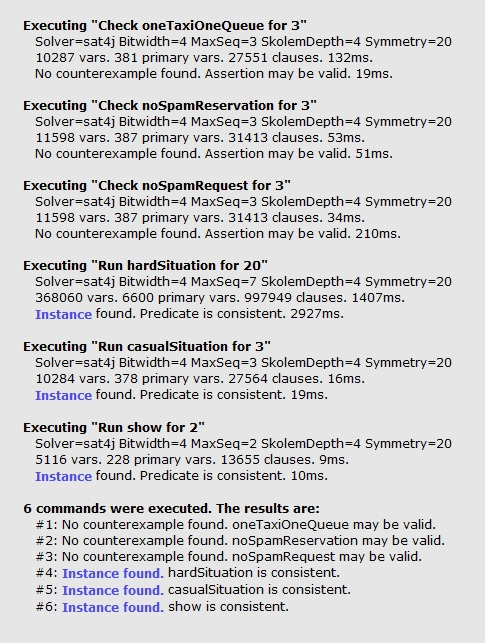
\includegraphics[scale=1]{../SE2_ALLOY/Answer}
			\caption{Alloy Answer}	
		\end{center}
	\end{figure}
	
	\subsection{Alloy Worlds}
		\subsubsection{Hard Situation}
		We do not insert the image for this test case because is huge and
		pretty incomprehensible. The test has been executed to ensure that the
		model keeps consisting also with a significant number of entities.
		\newpage
		\begin{landscape}
		\subsubsection{Casual Situation}
			\begin{figure}[!h]
				\begin{center}			
					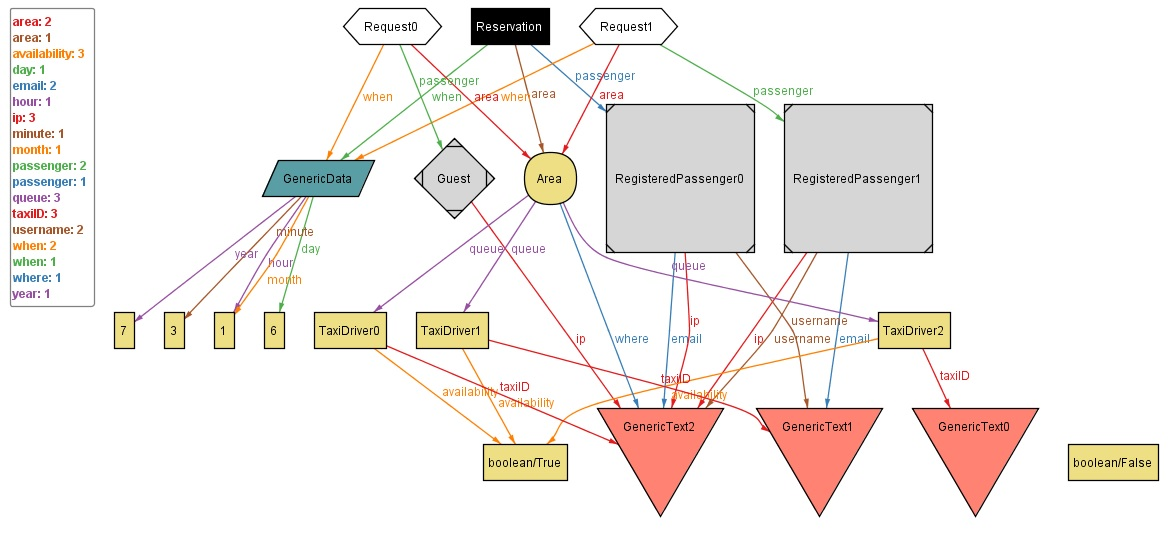
\includegraphics[height=0.75\textheight]{../SE2_ALLOY/CasualSituation}
					\caption{World Representation - Casual Situation}	
				\end{center}
			\end{figure}
		\end{landscape}
		\newpage
		\begin{landscape}
		\subsubsection{Show}
			\begin{figure}[!h]
				\begin{center}			
					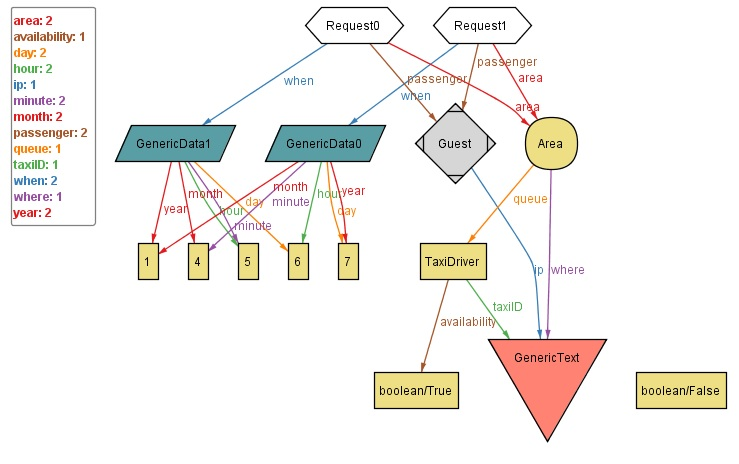
\includegraphics[height=0.75\textheight]{../SE2_ALLOY/Show}
					\caption{World Representation - Default Show}	
				\end{center}
			\end{figure}
		\end{landscape}